\documentclass[12pt]{article}
\newif\ifanswer\answertrue%\answerfalse% comment out to show/hide answers
\usepackage{../preamble3}% preamble always after \newif\ifanswer
\renewcommand{\theenumi}{\alph{enumi}}
%\pagenumbering{gobble}
\title{Flintridge Prep Summer School, Algebra II \\ June-July 2021}
\author{Patrick \& James Toche}
\date{Revised:~\today}

\begin{document}
\maketitle
\begin{minipage}{\textwidth}
\begin{abstract}\setlength{\parindent}{0pt}%
Notes on the Flintridge Prep Summer Course Algebra II.
Copyright restrictions may apply. Written for personal use. 
Please report typos and errors over at \url{https://github.com/ptoche/Math/tree/master/aops}. 
\end{abstract}
\end{minipage}

\thispagestyle{empty}
\clearpage


%%%%%%%%%%%%%%%%%%%%%%%%%%%%%%%%%%%%%%%%%%%%%%%%%%%%%%%%%%%%%%%%%%%%%%%%
\subsection*{1. (Problem Solving)}

\nopagebreak

After summer school is over, M. will go back to her job at the local health-food store, where one of the more challenging tasks she has to do is mixing juices for all the hipster customers who really dig mixed juice. She did a particular mix one day of ginger and apple juice. A cup of ginger juice costs $\$2.65$, and a cup of apple juice costs $\$1.98$. The first customer to come in can only afford to pay $\$18$ for $8$ cups of juice. How many cups of ginger and apple juice should M. use in the mixture, respectively? (round your answers to the nearest tenth of a cup) 

\begin{answer}
Let $A$ denote the quantity of Apple juice and $G$ the quantity of Ginger juice used in the mix (in units of ``cup''). The sum of these must equal $8$ cups. The total cost of the mix must be $\$18$ ($18/8=\$2.25$ per cup of mix). We have a linear system of two equations in two unknowns.
\begin{align*}
 2.65 G + 1.98 A & = 18 \\
           G + A & = 8
\end{align*}
We can solve for $G$ and $A$ by substitution:
\begin{align*}
 2.65 G + 1.98 (8 - G) & = 18 \\
           G & = \frac{18-8 \times 1.98}{2.65-1.98} = \frac{2.16}{0.67} \\
           G & \approx 3.2 \\
           A & \approx 4.8 \\
\end{align*}
\begin{empheq}[box={\mathbox[colback=white]}]{equation*}
    G = 3.2, \quad A = 4.8
\end{empheq} 
\end{answer}
%%%%%%%%%%%%%%%%%%%%%%%%%%%%%%%%%%%%%%%%%%%%%%%%%%%%%%%%%%%%%%%%%%%%%%%%

\iftoggle{showAnswers}{\newpage}


%%%%%%%%%%%%%%%%%%%%%%%%%%%%%%%%%%%%%%%%%%%%%%%%%%%%%%%%%%%%%%%%%%%%%%%%
\subsection*{2.}

\nopagebreak

The diagram shows a screen on which the lines $5x+4y=32$ and $-5x+6y=8$ have been graphed. The window settings for this diagram consist of two inequalities, $a\leq x\leq b$ and $c\leq y\leq d$, in which the numbers $a$, $b$, $c$, and $d$ are determined by the diagram. What are these numbers? 
\begin{center}
  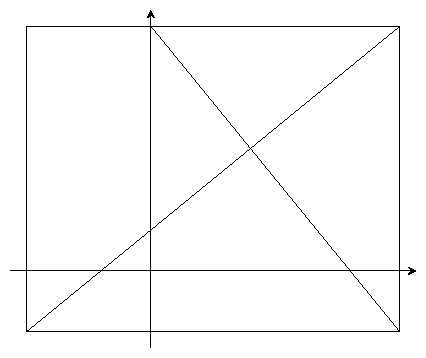
\includegraphics[height=4cm,page=1]{flintprep-problem-02}
\end{center}
\begin{answer}
First, place labels on the figure. 

\begin{center}
  \colorbox{white}{\includegraphics[height=9cm,page=2]{flintprep-problem-02}}
\end{center}

The top-left corner, at the $y$-coordinate $d$, is the intercept of the line with equation $5x+4y=32$. Thus, $d$ is the intercept of the line, and thus $d=8$. The top-right corner has the same $y$-coordinate $8$ and $x$-coordinate $b$ and lies on the line with equation $-5x+6y=8$. Thus the point $(b,8)$ must satisfy the equation, and thus $b=8$. We can go on to solve for all values as follows:
\begin{align*}
(0,d) \in \{5x + 4y = 32\} 
  & \quad\Rightarrow\quad
  5 \cdot 0 + 4 \cdot d = 32
  \quad\Rightarrow\quad
  d = 8 \\
(b,d) = (b,8) \in \{-5x + 6y = 8\} 
  & \quad\Rightarrow\quad
  -5 \cdot b + 6 \cdot 8 = 8
  \quad\Rightarrow\quad
  b = 8 \\  
(b,c) = (8,c) \in \{5x + 4y = 32\} 
  & \quad\Rightarrow\quad
  5 \cdot 8 + 4 \cdot c = 32
  \quad\Rightarrow\quad
  c = -2 \\
(a,c) = (a,-2) \in \{-5x + 6y = 8\} 
  & \quad\Rightarrow\quad
  -5 \cdot a + 6 \cdot (-2) = 8
  \quad\Rightarrow\quad
  a = -4
\end{align*}
\begin{empheq}[box={\mathbox[colback=white]}]{equation*}
    a = -4, \quad b = 8,  \quad c = -2,  \quad d = 8
\end{empheq} 
\end{answer}
%%%%%%%%%%%%%%%%%%%%%%%%%%%%%%%%%%%%%%%%%%%%%%%%%%%%%%%%%%%%%%%%%%%%%%%%

\iftoggle{showAnswers}{\newpage}

%%%%%%%%%%%%%%%%%%%%%%%%%%%%%%%%%%%%%%%%%%%%%%%%%%%%%%%%%%%%%%%%%%%%%%%%
\subsection*{3.}

\nopagebreak

A car went a distance of $90$km at a steady speed and returned along the same route at half that speed. The time needed for the whole round trip was four hours and a half. Find the two speeds. 

\begin{answer}
Since  velocity $v$ (speed) is defined over a short distance $d$ and duration $t$ as the ratio $d/t$, if we know both the duration and the constant velocity, we can calculate a distance as $d=vt$. Since the speed is constant over each trip, there are two regimes. Let $v_{1}, t_{1}$ denote velocity/duration for the first part of the trip and $v_{2},t_{2}$ for the second part. We know that $t_{1}+t_{2}=4.5$ hours and $v_{1}=v_{2}/2$. We also have $d_{1}=d_{2}=90$. Thus,
\begin{align*}
        v_{1} & = 2 v_{2} \\
t_{1} + t_{2} & = 4.5 \\
  v_{1} t_{1} & = 90\\
  v_{2} t_{2} & = 90
\end{align*}
This is a linear system of $4$ equations in $4$ unknowns. Eliminate $v_{1},v_{2}$ to get a two-equation system in $t_{1},t_{2}$, from which $v_{1}$ and $v_{2}$ can be recovered:
\begin{align*}
          v_{1} & = 2 v_{2} \\
          v_{2} & = 90/t_{2}\\
2 t_{1} - t_{2} & = 0 \\
  t_{1} + t_{2} & = 4.5
\end{align*}
Solution:
\begin{align*}
        t_{1} = 1.5, \quad
        t_{2} = 3,   \quad
        v_{1} = 60,  \quad
        v_{2} = 30
\end{align*}
\begin{empheq}[box={\mathbox[colback=white]}]{equation*}
        v_{1} = 60,\quad v_{2} = 30
\end{empheq} 
\end{answer}
%%%%%%%%%%%%%%%%%%%%%%%%%%%%%%%%%%%%%%%%%%%%%%%%%%%%%%%%%%%%%%%%%%%%%%%%

\iftoggle{showAnswers}{\newpage}

%%%%%%%%%%%%%%%%%%%%%%%%%%%%%%%%%%%%%%%%%%%%%%%%%%%%%%%%%%%%%%%%%%%%%%%%
\subsection*{4. Problem 293}

\nopagebreak

The Prep Ski club is planning a trip to Mammoth during semester break. They have $40$ skiers signed up to go, and the ski resort is charging $\$120$ for each person. 

\begin{enumerate}

\item 
Calculate how much money (revenue) the resort expects to take in.

\begin{answer}
\begin{align*}
40 \times \$120 = \$ 4800
\end{align*}
\end{answer}

\item 
The resort manager offers to reduce the group rate of $\$120$ per person by $\$2$ for each additional registrant, as long as the revenue continues to increase. For example, if $5$ more skiers sign up, all $45$ would pay $\$110$ each, producing revenue of $\$4950$ for the resort. Fill in the table for the manager. 

\begin{center}
\renewcommand{\arraystretch}{1.5}
\newcolumntype{C}[1]{>{\centering\arraybackslash}p{#1}} % centered 'p' col.
\begin{tabular}{*{4}{C{0.2\linewidth}}}
    \hline
    extras & persons & cost/person & revenue \\
    \hline
    $0$    &   $40$  &         &  \\
    $1$    &   $41$  &         &  \\
    $2$    &   $42$  &         &  \\
    $3$    &   $43$  &         &  \\
    $4$    &   $44$  &  $110$  & $4950$\\
    $5$    &   $45$  &         &  \\
    $6$    &   $46$  &         &  \\
    $7$    &   $47$  &         &  \\
    $8$    &   $48$  &         &  \\
    $9$    &   $49$  &         &  \\
    $10$   &   $50$  &         &  \\
    $11$   &   $51$  &         &  \\
    $12$   &   $52$  &         &  \\
    \hline
    \end{tabular}
\end{center}


\begin{answer}
\begin{center}
\renewcommand{\arraystretch}{1.5}
\newcolumntype{C}[1]{>{\centering\arraybackslash}p{#1}} % centered 'p' col.
\begin{tabular}{*{4}{C{0.2\linewidth}}}
    \hline
    extras & persons & cost/person & revenue \\
    \hline
    $0$    &   $40$  &   $120$  &   $4800$\\
    $1$    &   $41$  &   $118$  &   $4838$\\
    $2$    &   $42$  &   $116$  &   $4872$\\
    $3$    &   $43$  &   $114$  &   $4902$\\
    $4$    &   $44$  &   $112$  &   $4928$\\
    $5$    &   $45$  &   $110$  &   $4950$\\
    $6$    &   $46$  &   $108$  &   $4968$\\
    $7$    &   $47$  &   $106$  &   $4982$\\
    $8$    &   $48$  &   $104$  &   $4992$\\
    $9$    &   $49$  &   $102$  &   $4998$\\
    $10$   &   $50$  &   $100$  &   $5000$\\
    $11$   &   $51$  &    $98$  &   $4998$\\
    $12$   &   $52$  &    $96$  &   $4992$\\
    \hline
    \end{tabular}
\end{center}

\end{answer}

\item 
Let $x$ be the number of new registrants. In terms of $x$, write expressions for the total number of persons going, the cost to each, and the resulting revenue for the resort.

\begin{answer}
\begin{align*}
\text{number of persons} &: 40 + x\\
\text{cost per person} &: 120 - 2x\\
\text{total revenue} &: (120 - 2x) (40 + x)
\end{align*}
\end{answer}

\item 
Plot your revenue values versus $x$, for the relevant values of $x$. Because this is a discrete problem, it does not make sense to connect the dots. 

\begin{answer}
Revenue is a quadratic function of the number of new registrants $x$.
\begin{align*}
(120 - 2x) (40 + x) 
& = - 2x^2 + 40x + 4800 \\
& = - 2 (x^2 - 20x - 2400) \\
& = - 2 ((x - 10)^2 - 100 - 2400) \\
& = - 2 ((x - 10)^2 - 50^2) \\
& = - 2 (x - 10 - 50)(x - 10 + 50) \\
& = - 2 (x - 60)(x + 40) 
\end{align*}
Revenue starts at $40 \times \$120 = \$4800$ for $x=0$, rises then falls to $0$ for $x=60$. 

\begin{center}
  \colorbox{white}{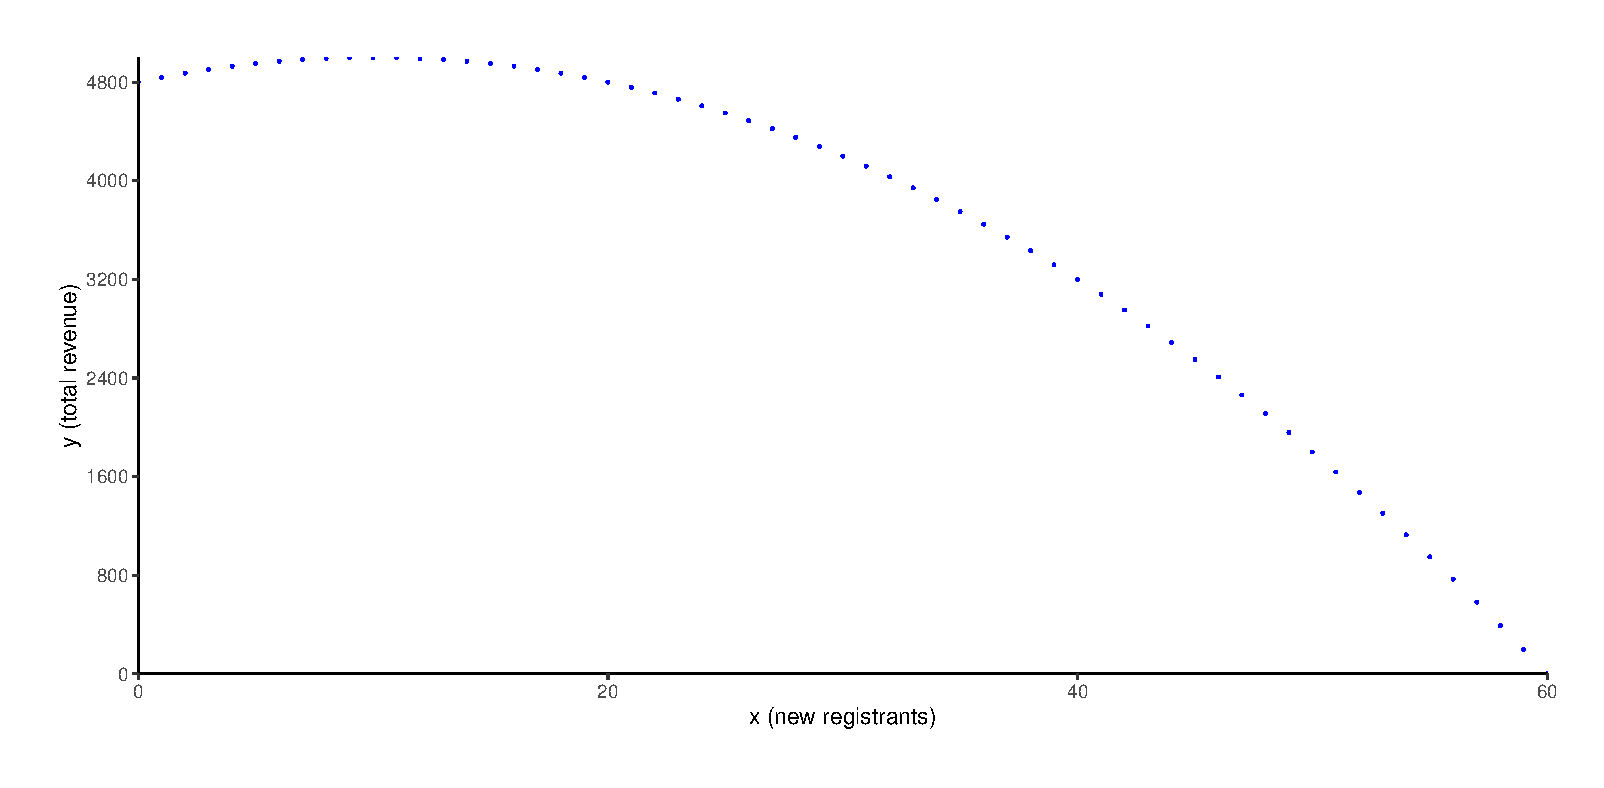
\includegraphics[width=0.95\linewidth]{flintprep-293}}
\end{center}

To see the big picture, we plot revenue in terms of the total number of registrants: Revenue starts at $0$, rises to a maximum for $50$ registrants, then falls to $0$ for $100$ registrants. 
\begin{center}
  \colorbox{white}{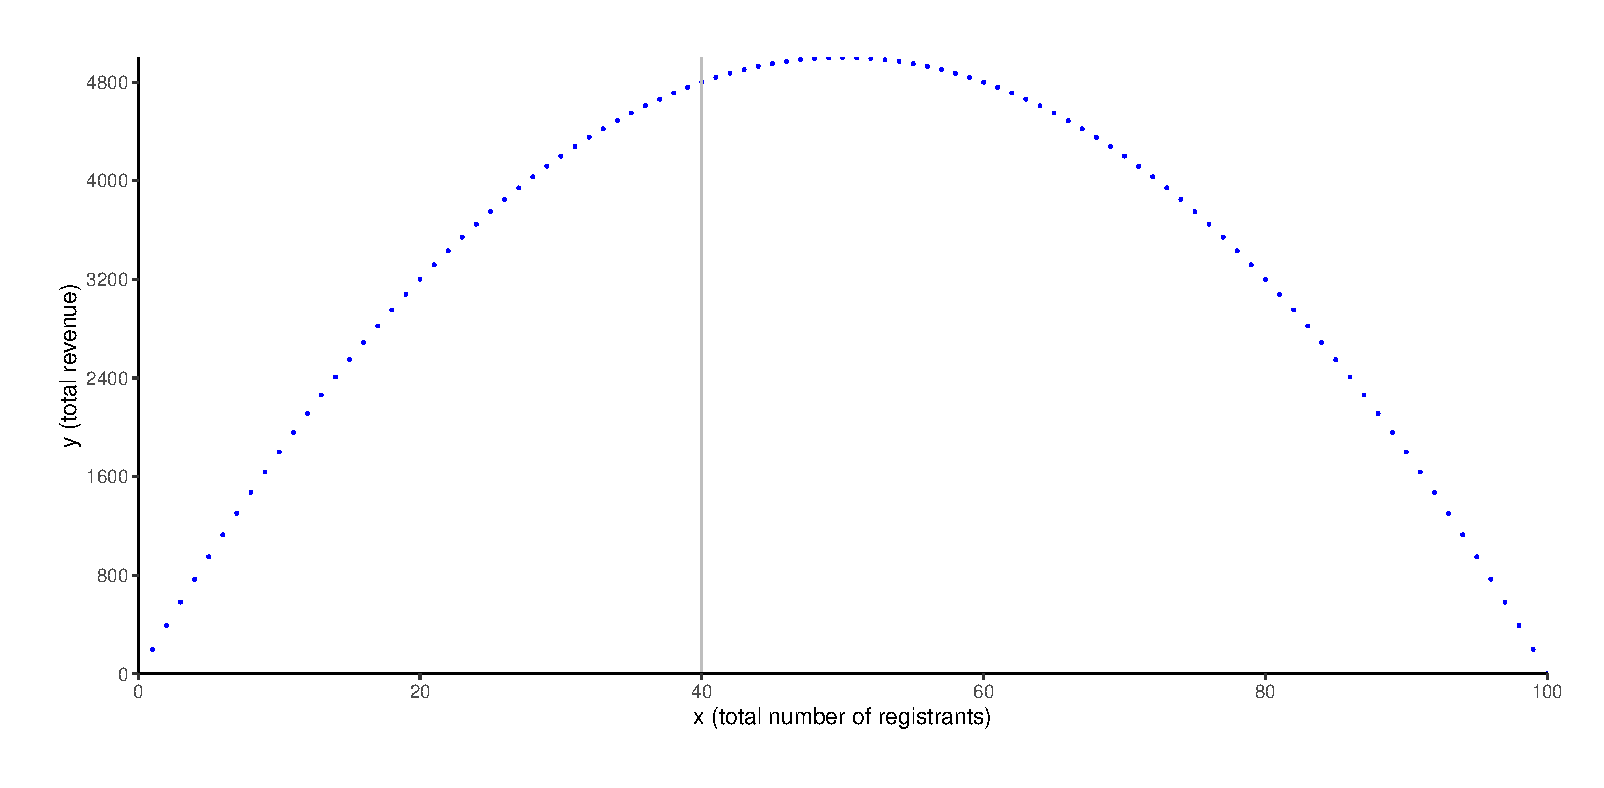
\includegraphics[width=0.95\linewidth]{flintprep-293-total}}
\end{center}
\end{answer}

\item 
For the resort to take in at least $\$4900$, how many skiers must go on the trip?

\begin{answer}
The condition on revenue is:
\begin{align*}
y = (120 - 2x) (40 + x) & \geq 4900
\end{align*}
Solve for $x$ when the inequality is strict:
\begin{align*}
    (120 - 2x) (40 + x) & = 4900 \\
          -2 x^2 + 40 x & = 100 \\
             x^2 - 20 x & = -50 \\
        (x-10)^2 - 10^2 & = -50 \\
     (x-10-\sqrt{50})(x-10+\sqrt{50}) & = 0
\end{align*}
The roots are approximately $17.07$ and $2.92$. The closest integers associated with revenue greater than $4900$ are $x=17$ and $x=3$. The corresponding revenues are:
\begin{align*}
x = 3:  & y = (120 - 2 \cdot 3) (40 + 3) = 4902 \\
x = 17: & y = (120 - 2 \cdot 17) (40 + 17) = 4902
\end{align*}
Any value in between generates even greater revenue. Thus, the resort can take in any number of new registrants between $3$ and $17$ or, equivalently, a total number skiers between $43$ and $57$. The maximal revenue is achieved for $x=10$ new registrants, or $50$ skiers, with a revenue of $y=\$5000$.
\end{answer}

\iftoggle{showAnswers}{\newpage}

%%%%%%%%%%%%%%%%%%%%%%%%%%%%%%%%%%%%%%%%%%%%%%%%%%%%%%%%%%%%%%%%%%%%%%%%
\subsection*{5. Question 11 of MidTerm Test}

\nopagebreak

After high school, N. gets a job at the fire department, and is in charge of operating the hose, which shoots water out in a parabolic arc. Assume the behavior of the hose can be modeled by quadratic function. The hose is sprayed from $4.5$ feet above ground, and hits the ground a horizontal distance of $58$ feet away. The maximum height of the water occurs $28$ feet from where the hose is sprayed. Let $x$ bet the horizontal distance from the hose nozzle, and $y$ be the corresponding height of the stream of water, both in feet. 

\begin{enumerate}

\item What is the quadratic equation that models the path of the water?

\begin{answer}
The general equation is
\begin{align*}
y = a x^2 + b x + c
\end{align*} 
where $a$, $b$, $c$ are constants to be determined. Obviously $a<0$ since the path of the water is up then down. The $y$ intercept is at $4.5$ feet, so $c=4.5$. One of the roots is at $x=58$, giving the condition
\begin{align*}
58^2 \cdot a + 58 \cdot b + 4.5 = 0
\end{align*}
a linear equation in the parameters $a$ and $b$. Since the maximum height occurs at $28$ feet, the vertex is located at $x=28$,
\begin{align*}
y & = a x^2 + b x + c \\
  & = a (x^2 + \frac{b}{a} x +  \frac{c}{a}) \\
  & = a \left[\left(x + \frac{b}{2a}\right)^2 - \left(\frac{b}{2a}\right)^2  + \frac{c}{a}\right] 
\end{align*}
The vertex condition gives:
\begin{align*}
x = - \frac{b}{2a} = 28
\quad\Rightarrow\quad 
b = -56a
\end{align*}

The parameters $a$ and $b$ satisfy the system:
\begin{align*}
58^2a + 58b + 4.5 & = 0 \\
56a + b & = 0 
\end{align*}
Subtracting $58$ times the second equation from the first eliminates $b$:
\begin{align*}
(58^2 - 58 \cdot 56) a + 4.5 & = 0 \\
\quad\Rightarrow\quad 
a & = -\frac{4.5}{116} 
  \approx 0.0043\\[1ex]
b & = \frac{56 \times 4.5}{116}
  = \frac{252}{116}
  = \frac{63}{29}
  \approx 2.1724
\end{align*}

The quadratic equation is:
\begin{align*}
y = -\frac{45}{1160} \cdot x^2 + \frac{63}{29} \cdot x + 4.5 
\end{align*}

\end{answer}

\item Graph the function.

\begin{answer}
\begin{center}
  \colorbox{white}{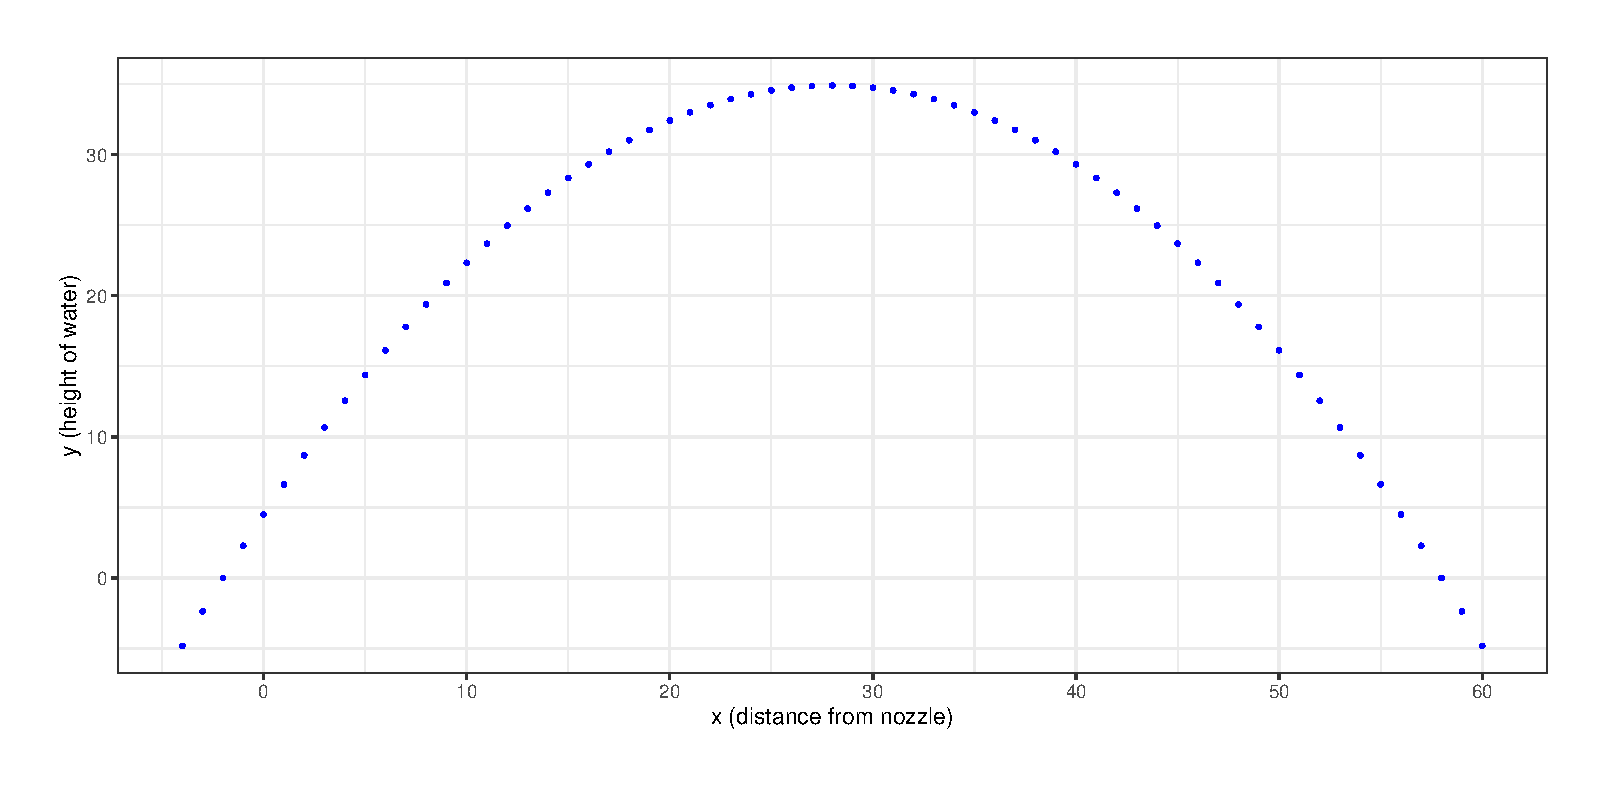
\includegraphics[width=0.95\linewidth]{flintprep-midterm-11}}
\end{center}
\end{answer}

\item What is the maximum height of the water?

\begin{answer}
The maximum height occurs for $x=28$:
\begin{align*}
y = -\frac{45}{1160} \cdot 28^2 + \frac{63}{29} \cdot 28 + 4.5 
  \approx 34.9
\end{align*} 
\end{answer}

\item Will the stream go over a $6$ ft high fence that is located $48$ feet from the nozzle? Explain your reasoning and show any work that is needed. 

\begin{answer}
The question is whether $y>6$ for $x=48$:
\begin{align*}
y = -\frac{45}{1160} \cdot 48^2 + \frac{63}{29} \cdot 48 + 4.5 
  \approx 19.4
\end{align*} 
The height of the water is more than three times greater than the fence. 
\end{answer}

\end{enumerate}
%%%%%%%%%%%%%%%%%%%%%%%%%%%%%%%%%%%%%%%%%%%%%%%%%%%%%%%%%%%%%%%%%%%%%%%%





\end{enumerate}
%%%%%%%%%%%%%%%%%%%%%%%%%%%%%%%%%%%%%%%%%%%%%%%%%%%%%%%%%%%%%%%%%%%%%%%%

\iftoggle{showAnswers}{\newpage}

\end{document}


%%%%%%%%%%%%%%%%%%%%%%%%%%%%%%%%%%%%%%%%%%%%%%%%%%%%%%%%%%%%%%%%%%%%%%%%
\subsection*{1.}

\nopagebreak

a
\begin{answer}
a
\begin{align*}
x
\end{align*}
\begin{empheq}[box={\mathbox[colback=white]}]{equation*}
    x
\end{empheq} 
\end{answer}
%%%%%%%%%%%%%%%%%%%%%%%%%%%%%%%%%%%%%%%%%%%%%%%%%%%%%%%%%%%%%%%%%%%%%%%%

\iftoggle{showAnswers}{\newpage}














%% TO DO TO DO TO DO TO DO TO DO


%%%%%%%%%%%%%%%%%%%%%%%%%%%%%%%%%%%%%%%%%%%%%%%%%%%%%%%%%%%%%%%%%%%%%%%%
\subsection*{4. Inspired by Problem 293}

\nopagebreak

The Prep Ski club is planning a trip to Mammoth during semester break. They have $40$ skiers signed up to go, and the ski resort is charging $\$120$ for each person. The resort manager needs at least $10$ new skiers to sign up to make the trip profitable. He offers to reduce the individual rate of $\$120$ per person by $\$2$ for each new registrant, as long as the revenue continues to increase. For example, the $41$st skier to sign up would pay $\$118$, the $42$nd skier would pay $\$116$. See the table:

\begin{center}
\renewcommand{\arraystretch}{1.5}
\newcolumntype{C}[1]{>{\centering\arraybackslash}p{#1}} % centered 'p' col.
\begin{tabular}{*{4}{C{0.2\linewidth}}}
    \hline
    extras & persons & cost/person & revenue \\
    \hline
    $0$    &   $40$  &      $120$  &   $4800$\\
    $1$    &   $41$  &      $118$  &  \\
    $2$    &   $42$  &      $116$  &  \\
    $3$    &   $43$  &             &  \\
    $4$    &   $44$  &             &  \\
    $5$    &   $45$  &             &  \\
    $6$    &   $46$  &             &  \\
    $7$    &   $47$  &             &  \\
    $8$    &   $48$  &             &  \\
    $9$    &   $49$  &             &  \\
    $10$   &   $50$  &             &  \\
    $11$   &   $51$  &             &  \\
    $12$   &   $52$  &             &  \\
    \hline
    \end{tabular}
\end{center}

\begin{enumerate}

\item 
Fill in the table for the manager. 

\begin{answer}
\begin{center}
  \colorbox{white}{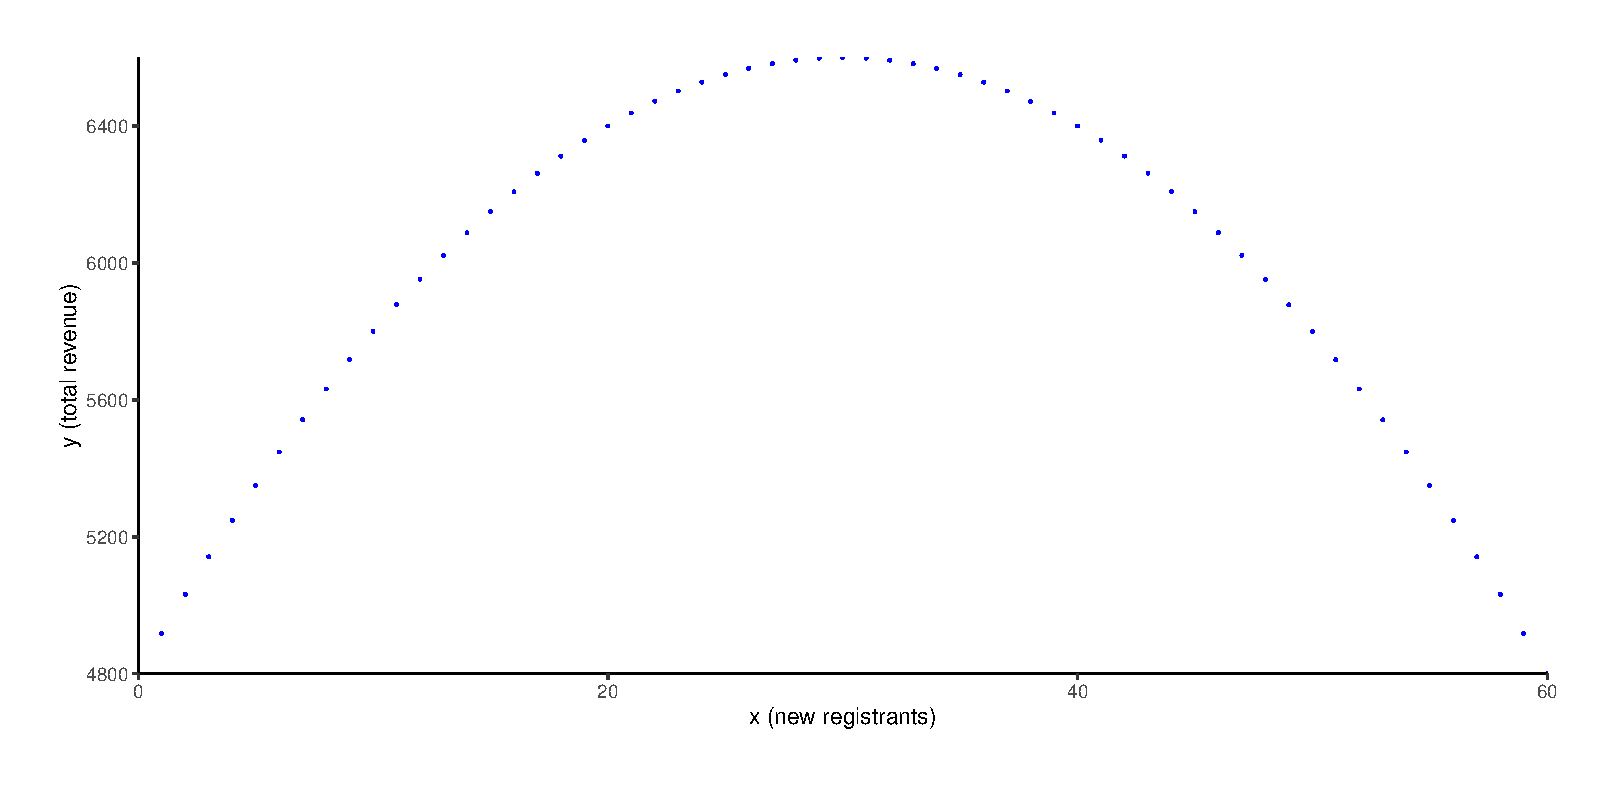
\includegraphics[width=0.95\linewidth]{flintprep-293-variant-1}}
\end{center}
\begin{center}
  \colorbox{white}{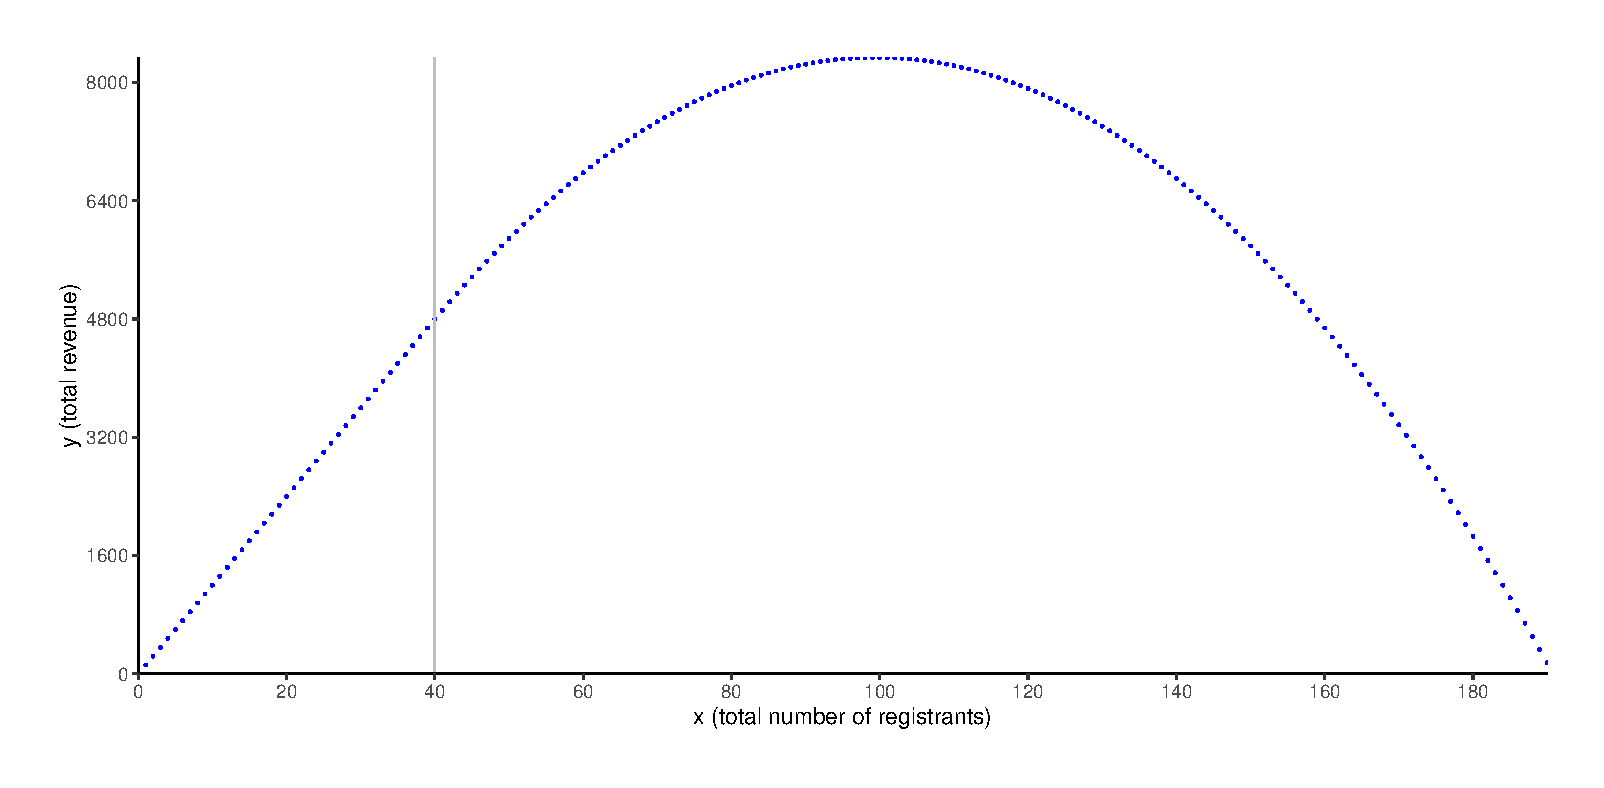
\includegraphics[width=0.95\linewidth]{flintprep-293-variant-2}}
\end{center}
\end{answer}

\item 
Let $n$ be the total number of registrants. Write an expression for revenue in terms of $n$ and plot it. 

\begin{answer}
\end{answer}

\item
For the resort to take in at least $\$4900$, how many skiers must go on the trip?

\begin{answer}
\end{answer}

\end{enumerate}

\iftoggle{showAnswers}{\newpage}